\documentclass{article}
\usepackage{amsmath}
\usepackage{tikz}
\usetikzlibrary{matrix,arrows}

\begin{document}

\section*{Semigroup $U_2$: Posets of Classes}

For the semigroup $U_2$, the posets of \textit{${\mathcal{L}}$}-classes (left), \textit{${\mathcal{R}}$}-classes (middle left), \textit{${\mathcal{J}}$}-classes (middle right), and \textit{${\mathcal{H}}$}-classes (right).

\begin{figure}[h]
    \centering
    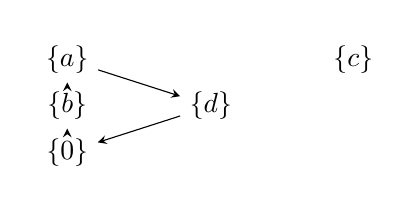
\begin{tikzpicture}[baseline=-0.6ex]
        \matrix (m) [matrix of math nodes,row sep=0em,column sep=3em,minimum width=1.5em] {
            \{a\} &  & \{c\} \\
            \{b\} & \{d\} \\
            \{0\} &  \\
        };
        \path[-stealth]
        (m-1-1) edge node [left] {} (m-2-1)
                edge node [right] {} (m-2-2)
        (m-2-1) edge node [above] {} (m-3-1)
        (m-2-2) edge node [above] {} (m-3-1);
    \end{tikzpicture}\quad
    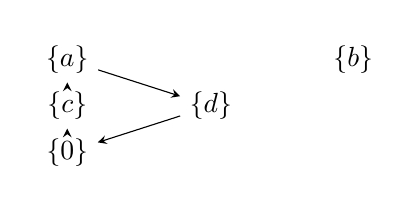
\begin{tikzpicture}[baseline=-0.6ex]
        \matrix (m) [matrix of math nodes,row sep=0em,column sep=3em,minimum width=1.5em] {
            \{a\} &  & \{b\} \\
            \{c\} & \{d\} \\
            \{0\} &  \\
        };
        \path[-stealth]
        (m-1-1) edge node [left] {} (m-2-1)
                edge node [right] {} (m-2-2)
        (m-2-1) edge node [above] {} (m-3-1)
        (m-2-2) edge node [above] {} (m-3-1);
    \end{tikzpicture}\quad
    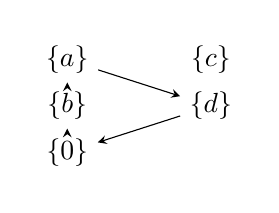
\begin{tikzpicture}[baseline=-0.6ex]
        \matrix (m) [matrix of math nodes,row sep=0em,column sep=3em,minimum width=1.5em] {
            \{a\} & \{c\} \\
            \{b\} & \{d\} \\
            \{0\} &  \\
        };
        \path[-stealth]
        (m-1-1) edge node [left] {} (m-2-1)
                edge node [right] {} (m-2-2)
        (m-2-1) edge node [above] {} (m-3-1)
        (m-2-2) edge node [above] {} (m-3-1);
    \end{tikzpicture}\quad
    \begin{tikzpicture}[baseline=-0.6ex]
        \matrix (m) [matrix of math nodes,row sep=0em,column sep=3em,minimum width=1.5em] {
            \{a\} & \{b\} \\
            \{0\} &  \\
            \{c\} & \{d\} \\
        };
        \path[-stealth]
        (m-1-1) edge node [left] {} (m-2-2)
        (m-1-1) edge node [right] {} (m-3-2)
        (m-1-2) edge node [left] {} (m-2-2)
        (m-1-2) edge node [right] {} (m-3-2)
        (m-2-2) edge node [above] {} (m-3-1)
        (m-2-2) edge node [above] {} (m-3-2);
    \end{tikzpicture}
\end{figure}

\end{document}